\chapter{Metodolog\'ia}

En el cap\'itulo anterior se explic\'o sobre las metodolog\'ias recientes que se 
utilizan para que un robot pueda ser aut\'onomo y genere un mapa 
del entorno donde se encuentre. En este trabajo de tesis se propone 
el movimiento aut\'onomo basado en campos potenciales y en leyes de control 
polar para el movimiento de un robot m\'ovil, de modo que sea capaz de alcanzar 
un objetivo que vuelva a planificar continuamente su camino sin colisiones. El 
algoritmo desarrollado puede ser implementado desde una computadora en tiempo 
real (\textit{online}) o tambi\'en puede ser implementado por medio de un 
microcontrolador (\textit{onboard}). En este cap\'itulo se explicar\'a, con detalles, 
los m\'etodos que fueron implementados en este trabajo.

\section{Prototipo a Utilizar}
En esta secci\'on se explicar\'a cada uno de los componentes que tuvo que 
ser utilizados para realizar la autonom\'ia y el mapeo de este trabajo de 
tesis. Para realizar la autonom\'ia se utiliz\'o un robot m\'ovil diferencial 
terrestre, y as\'i tambi\'en para mapear el entorno por donde el robot se 
desplaza se utiliz\'o un sensor Lidar.

%\subsection{Descripci\'on del Robot M\'ovil}
% \begin{figure}%[h]
% \centering \footnotesize
% {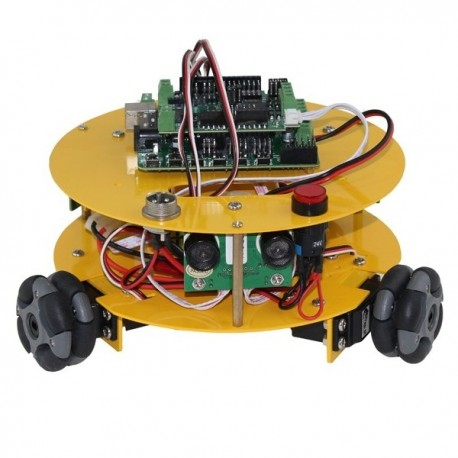
\includegraphics[width=0.40\linewidth]{images/omnidirecional.jpg}}
% \captionsetup{font=footnotesize}
% \caption{Robot m\'ovil hol\'onomico omnidireccional}
% \label{fig:omnidirectional}
% \end{figure}
% \begin{figure}%[h]
% \centering \footnotesize
% {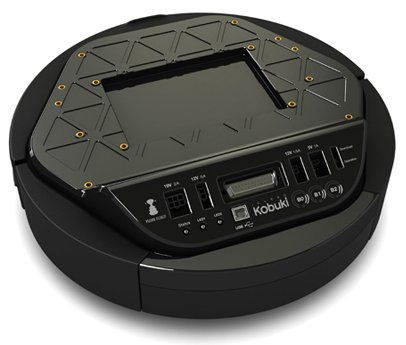
\includegraphics[width=0.40\linewidth]{images/kobuki.jpg}}
% \captionsetup{font=footnotesize}
% \caption{Robot m\'ovil no-hol\'onomico utilizado para implementar el 
% algoritmo de autonom\'ia}
% \label{fig:kobuki}
% \end{figure}
% Una forma de clasificar a los robots m\'oviles es a trav\'es de la locomoci\'on 
% de sus ruedas, esto se divide en dos: (1) robot holon\'omico y (2) robot 
% no-holon\'omico. El robot holon\'omico no tiene ninguna restricci\'on, con 
% respecto a la velocidad, en la posici\'on y la orientaci\'on. El robot se puede 
% mover instant\'aneamente en cualquier direcci\'on del espacio, sin necesidad de 
% rotar previamente. La mayor\'ia de estos robots m\'oviles son omnidireccionales, 
% como se puede ver en la figura \ref{fig:omnidirectional}. En cambio un robot 
% no-holonomico tiene una restricci\'on en su velocidad, no existe un trayectoria 
% que dependa solamente de la posici\'on y orientaci\'on. Por ende, este robot no 
% se puede mover instant\'aneamente en cada direcci\'on del espacio.

%Para este trabajo se hizo uso del robot m\'ovil no-holon\'omico, Kobuki (figura \ref{fig:kobuki})
%el cual esta configurado para poder trabajar con ROS (\textit{Robot Operating System}) 
%con una velocidad de translaci\'on de 70 $cm/s$, una velocidad de rotaci\'on de 180 
%$grados/s$, una posibilidad de carga de hasta 5 $kg$, un tiempo de operaci\'on de 3 
%horas \cite{aboutKobuki}. 

\subsection{Cinem\'atica de Robot M\'ovil Diferencial}
\begin{figure}%[h]
\centering \footnotesize
{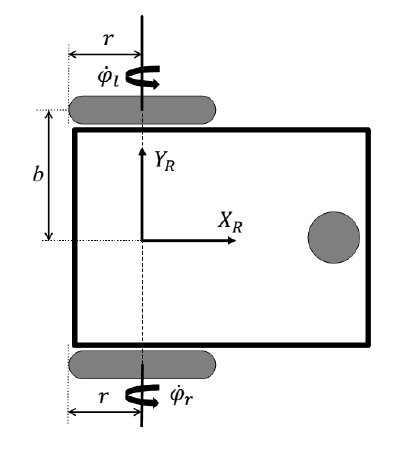
\includegraphics[width=0.40\linewidth]{images/kinematic_model.png}}
\captionsetup{font=footnotesize}
\caption{Representaci\'on gr\'afica de un robot m\'ovil diferencial. Donde 
$b$ es la distancia de su centro de masa hacia sus ruedas, el radio de cada 
rueda es representado por $r$. Finalmente $\dot{\varphi_{l}}$ y 
$\dot{\varphi_{r}}$ son las velocidades de la rueda derecha y rueda izquierda 
correspondientemente.}
\label{fig:RMkinematic}
\end{figure}
Para realizar el modelo del cinem\'atico del robot diferencial se debe tener 
en cuenta algunas consideraciones sobre el comportamiento de este. Se asume 
que el robot se desplaza en una superficie plana idealmente sin rozamiento, 
tambi\'en se toman los ejes de las ruedas como perpendiculares al suelo
por donde se desplaza y finalmente que solo existe un punto de contacto entre 
la rueda y el suelo.

%El robot se considera como un cuerpo r\'igido sin partes flexibles, pero se 
%deben tener en cuenta las restricciones no-holon\'omicas. Es decir, el robot 
%puede desplazarse hacia atr\'as o hacia adelante, pero no puede trasladarse 
%hacia los lados. Para poder realizar estos movimientos, se debe realizar un 
%movimiento en partes.

El modelo cinem\'atico del robot necesita conocer las dimensiones del robot. Las 
medidas que se necesitan son la distancia entre las ruedas y el radio de las 
mismas. La distancia entre las ruedas ser\'a representada como $2b$ y el radio de 
las ruedas como $r$. Tambi\'en se debe considerar que el robot tiene dos ruedas 
convencionales fijas y el sistema de referencia del robot se encuentra entre 
ambas ruedas, como se ve en la figura \ref{fig:RMkinematic}.

Teniendo en consideración las restricciones de las ruedas convencionales se halla la cinemática 
directa del robot móvil. La cinemática directa consiste en:
\begin{align*}
\dot{x}^{R} &= \frac{r}{2}(\dot{\varphi_{r}} + \dot{\varphi_{l}}) \\
\dot{\theta} &= \frac{r}{2b}(\dot{\varphi_{r}} + \dot{\varphi_{l}})
\end{align*}
donde $\dot{x}^{R}$ es la velocidad lineal y $\dot{\theta}$ es la velocidad angular. Estas 
velocidades del robot móvil se hallan a 
través de las velocidades de cada rueda del robot. Por otro lado la cinemática inversa 
como dice su nombre es todo lo contrario a la cinemática directa. Este consiste en:
\begin{align*}
\dot{\varphi_{r}} &= \frac{1}{r}(\dot{x}^{R} + b\dot{\theta}) \\
\dot{\varphi_{l}} &= \frac{1}{r}(\dot{x}^{R} - b\dot{\theta})
\end{align*}
donde se halla las velocidades de las ruedas a partir de la velocidad lineal y velocidad
angular del robot móvil.
\begin{figure}%[h]
 \centering \footnotesize
 {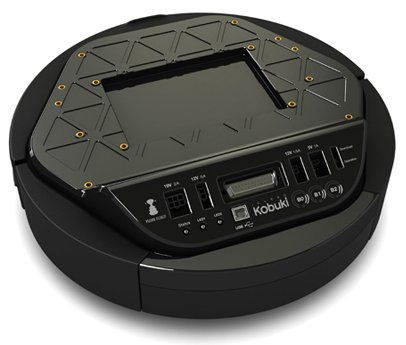
\includegraphics[width=0.35\linewidth]{images/kobuki.jpg}}
 \captionsetup{font=footnotesize}
 \caption{Robot m\'ovil utilizado para la implementación del algoritmo 
 de autonom\'ia}
 \label{fig:kobuki}
 \end{figure}
Para este trabajo se hizo uso del robot m\'ovil no-holon\'omico, Kobuki (figura \ref{fig:kobuki})
el cual trabaja con una velocidad de translaci\'on de 70 $cm/s$ y una velocidad de rotaci\'on 
de 180 $grados/s$. Tiene una posibilidad de carga de hasta 5 $kg$ y un tiempo de operaci\'on 
de 3 horas \cite{aboutKobuki}.
%Para calcular la cinem\'atica del robot m\'ovil se debe usar las restricciones 
%de las ruedas convencionales. Las restricciones de cada rueda fija son:
%\begin{equation*}
%\[-\text{sin}(\alpha + \beta) & \text{cos}(\alpha + \beta) & \text{lcos}(\beta)\] 
%{R}^R_{I} {I}^\dot{\xi} - r\dot{\varphi} &= 0 \\
%\[\text{cos}(\alpha + \beta) & \text{sin}(\alpha + \beta) & \text{lsin}(\beta)\]
%{R}^R_{I} {I}^\dot{\xi} &= 0
%\end{equation}
%donde ${R}^R_{I}$ es la matriz de rotaci\'on que lleva el sistema de coordenadas del 
%robot $(X_{R},Y_{R})$ al sistema inercial $(X_{I},Y_{I})$ y $\dot{\xi}$ 
%es el vector que contiene los valores de las velocidades lineales y angular 
%del robot.


\subsection{Sistema de Percepci\'on en 2D}
Para generar el mapa de un entorno, se necesita medir distancias del ambiente y así
generar el mapa. En este trabajo se utiliza un sensor lidar RPLidar A2 el cual se basa en 
el principio de rango de triangulación láser \cite{amann2001laser} y ha sido desarrollado 
por la empresa \textit{SLAMTEC}.

El sensor lidar es un sensor que no necesita tener una luz externa para poder obtener las
medidas de las distancias. Este sensor tiene un láser infrarrojo de baja potencia el cual
es controlado por medio de un pulso modulado. Este sensor puede girar en 360\grad ~y tiene
un rango de alcance máximo de 8 metros. Trabaja a una frecuencia de 10Hz teniendo una tasa 
de medición de 4000 muestras por segundo. La transmisión de datos de este sensor es por 
medio de un protocolo UART. El sensor es mostrado en la figura \ref{f:lidar}.


%Es un sensor l\'aser que se basa en el  principio de rango de triangulaci\'on 
%láser \cite{amann2001laser} y adopta el hardware de adquisici\'on y 
%procesamiento de visi\'on de alta velocidad desarrollado por \textit{SLAMTEC}. El 
%sensor utiliza un l\'aser infrarrojo de baja potencia como su fuente de luz y lo 
%maneja utilizando un pulso modulado. Este sensor gira a 360 \grad ~y llega a 
%una distancia m\'axima de 8 metros. Trabaja a una frecuencia de 10 Hz y 
%tiene una tasa de medici\'on de 4000 muestras por segundo. El hardware del 
%RPLIDAR A2 se puede ver en la figura \ref{f:lidar}, el cual tiene un 
%convertidor de protocolo UART a mini USB.
\begin{figure}%[h]
\centering \footnotesize
 {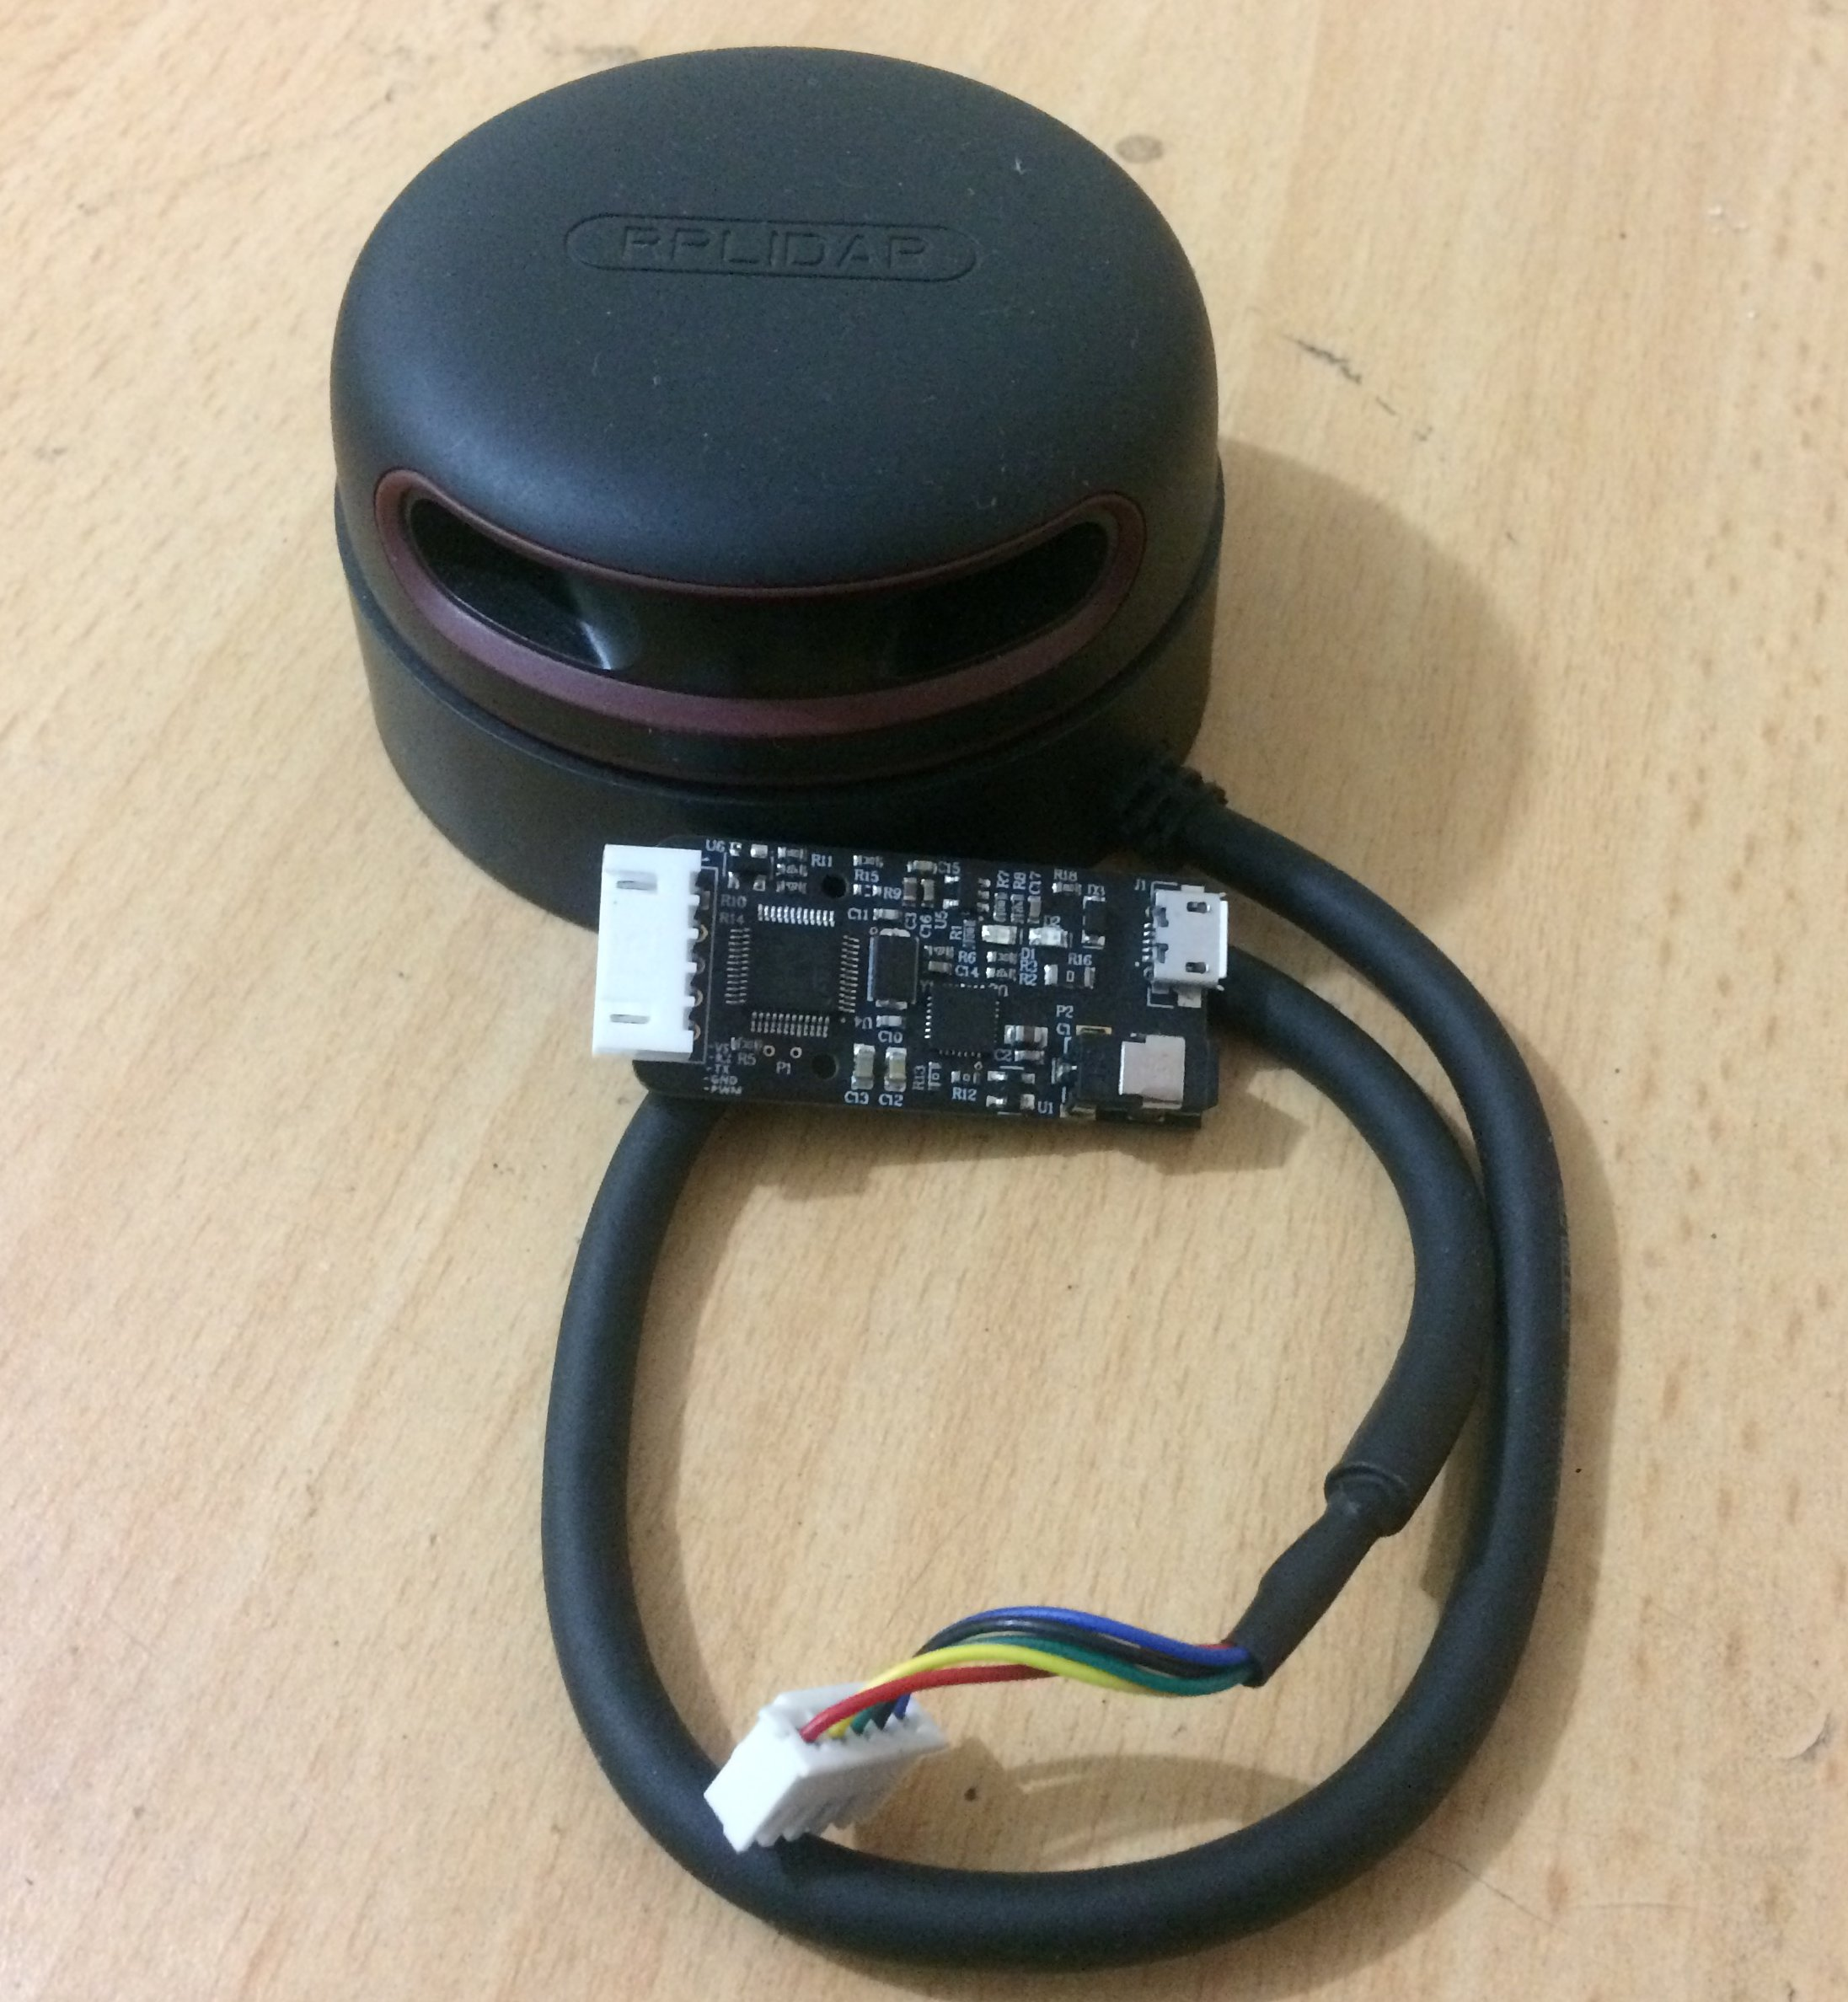
\includegraphics[width=0.60\linewidth]{images/rplidar.JPG}}
 \captionsetup{font=footnotesize}
 \caption{Sensor láser RPLIDAR A2.}
 \label{f:lidar}
\end{figure}

\begin{table}[htbp]
\begin{center}
\begin{tabular}{|l|c|c|c|c|}
\hline
Item & Unidad & M\'inimo & T\'ipico & M\'aximo\\
\hline \hline
Rango de distancia & m & 0.15 & - & 8 \\ \hline
Rango angular & grados & - & 0 - 360 & - \\ \hline
Resoluci\'on de la distancia & mm & - & menor a 0.5 & - \\ \hline
Duraci\'on de muestra & ms & - & 0.25 & - \\ \hline
Resoluci\'on angular & grados & 0.45 & 0.9 & 1.35 \\ \hline
Fecuencia de muestreo & Hz & 2000 & 4000 & 4100 \\ \hline
Frecuencia de escaneo & Hz & 5 & 10 & 15 \\ \hline
\end{tabular}
\caption{Pruebas de Medici\'on.}
\label{tbl:medicion}
\end{center}
\end{table}

La tabla \ref{tbl:medicion} muestra el rendimiento de medici\'on del 
sensor l\'aser \cite{Slamtec} considerando varias pruebas por cada item. Los items más 
importantes de esta tabla son: (1) Rango de distancia, el sensor toma mediciones en el
rango mostrado, cuando la distancia es menor a 0.15 $mts$ no considera la medición, lo 
mismo sucede cuando la medición es mayor a 8 $mts$. (2) Resolución de la distancia, el 
sensor tiene un error menor a 0.5 $mm$ en sus mediciones, esto permite construir un mapa 
con las dimensiones reales del entorno. (3) Resolución angular, este sensor tiene una 
resolución de 1\grad~ esto quiere decir que por cada grado que gira el lidar esta 
realizando una medición, por lo tanto el sensor mide 360 veces por cada rotación.

Para el envío de los datos a la PC o el microcontrolador, el sensor trabaja con un protocolo
de comunicación UART. Este protocolo se especifíca en la tabla \ref{tbl:comunicacion} y 
por medio de este se obtiene las distancias que mide el sensor. Para realizar el mapa en 
dos dimensiones, estas distancias tienen que convertirse en posiciones dentro del plano 
cartesiano por medio de una conversión de coordenas polares a coordenadas cartesianas.
\begin{table}[htbp]
\begin{center}
\begin{tabular}{|c|c|c|c|c|c|}
\hline
Color & Nombre de la se\~nal & Tipo & M\'inimo & T\'ipico & M\'aximo \\ 
\hline \hline
Rojo & VCC & Potencia & 4.9V & 5V & 5.5V \\ \hline
Amarillo & Tx & Salida & 0V & 3.3V & 3.5V \\ \hline
Verde & Rx & Entrada & 0V & 3.3V & 3.5V \\ \hline
Negro & GND & Potencia & 0V & 0V & 0V \\ \hline
Azul & MOTOCTL & Entrada & 0V & 3.3V & 5V \\ \hline
\end{tabular}
\caption{Interfaz de comunicaci\'on del sensor l\'aser.}
\label{tbl:comunicacion}
\end{center}
\end{table}

\subsection{Sistema de Percepci\'on en 3D}
\begin{figure}%[ht!]
  \centering \footnotesize
  %\subfloat[Attractive Force]{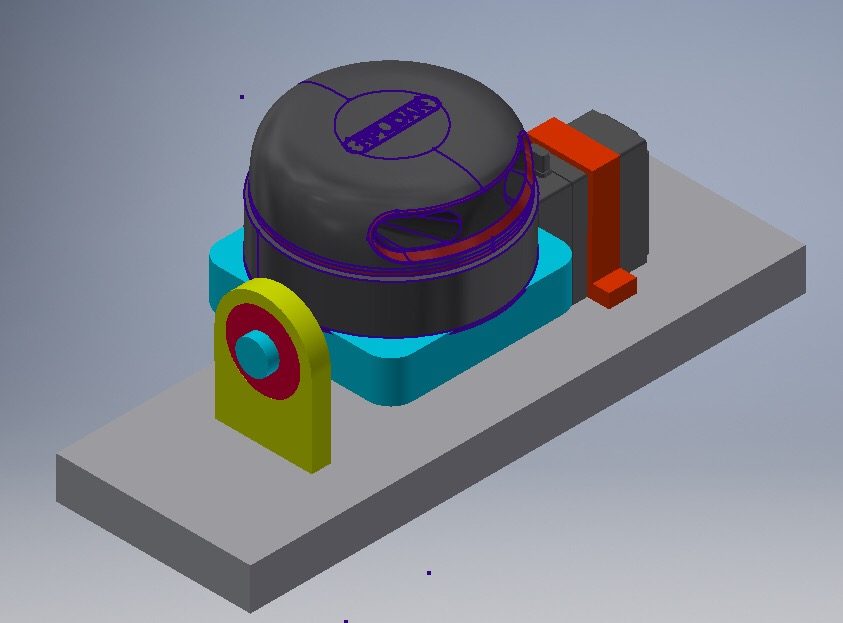
\includegraphics[width=0.16\textwidth]{images/lidar_3D.jpeg}}
  %~\subfloat[Repulsive Force]{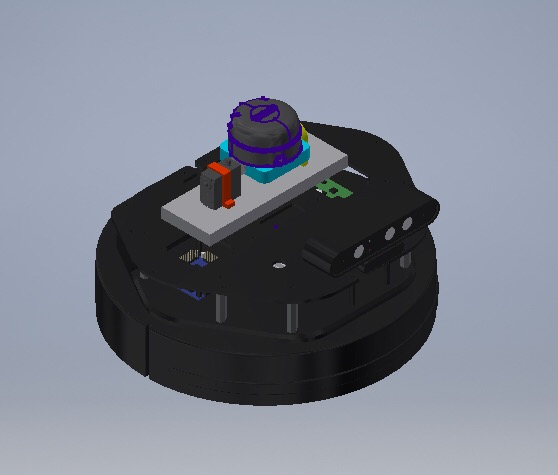
\includegraphics[width=0.16\textwidth]{images/kbki_lidar3D.jpeg}} 
  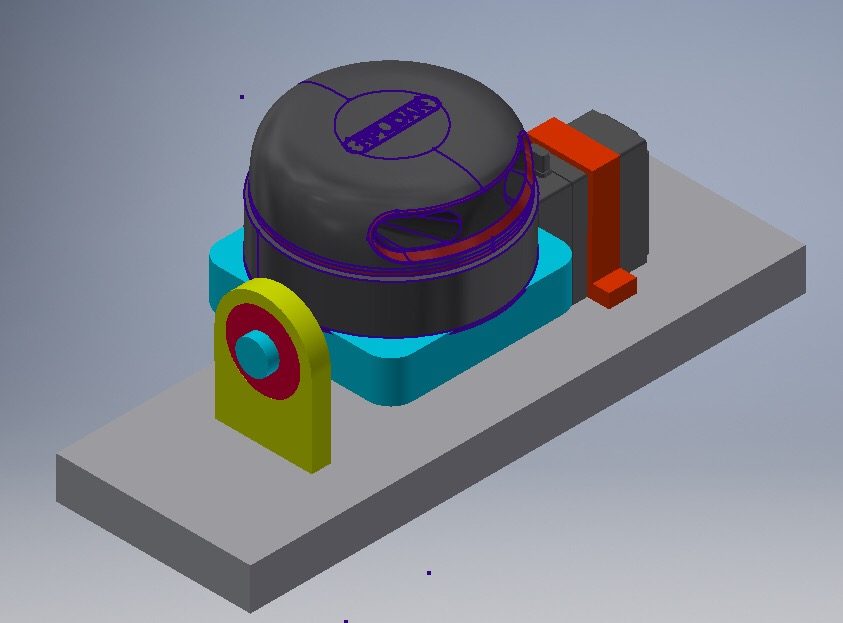
\includegraphics[width=0.40\textwidth]{images/lidar_3D.jpeg}
  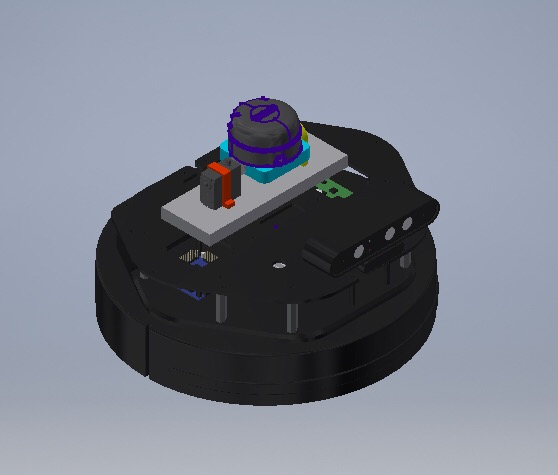
\includegraphics[width=0.35\textwidth]{images/kbki_lidar3D.jpeg}
  \\ $\qquad\qquad$ a. Sistema mecánico  $\qquad\qquad\qquad$  b. Sistema mecánico encima del Kobuki
  %\subfloat[Navigation Force]{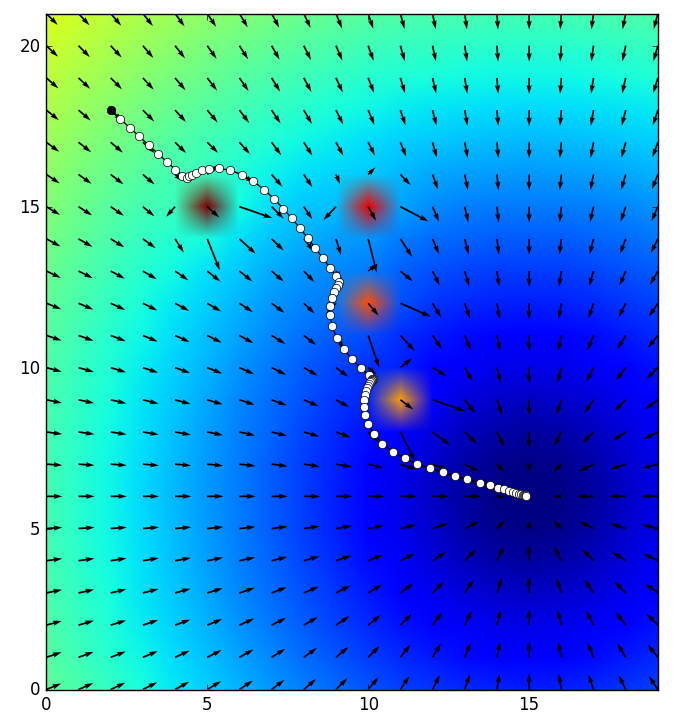
\includegraphics[width=0.16\textwidth]{images/nav_force.png}}
  % \subfloat[Attractive Force]{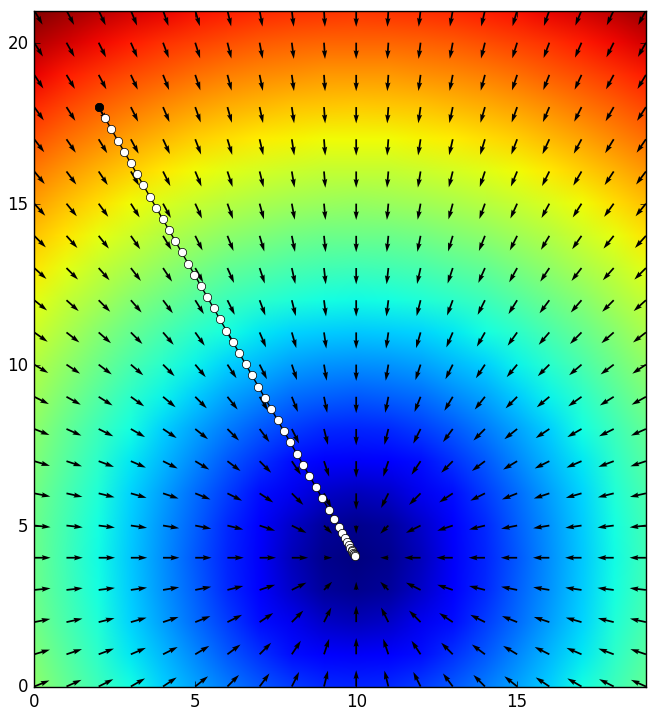
\includegraphics[width = 150mm]{attr_force.png}}
  \captionsetup{font=footnotesize}
  \caption{Sistema mec\'anico para el mapeo en tres dimensiones.}
  \label{f:lidar3D}
\end{figure}
El sensor lidar permite construir mapas en dos dimensiones ya que este va midiendo 
distancias mientras va rotando en 360\grad ~, pero para el alcance de este proyecto de 
tesis se necesita que el robot pueda mapear el entorno en tres dimensiones. Para este
objetivo se realizó un diseño mecánico, como se muestra en la figura \ref{f:lidar3D} (a). Este
diseño permite que el sensor lidar pueda tener un ángulo de medición de $\pm$ 15\grad. El sistema
mecánico consiste en una base que esta acoplada al sensor lidar, esta base se encuentra unida
a un eje junto a un servomotor. El servomotor esta programado para que se mueva en un rango de
$\pm$ 15\grad~ permitiendo que el sensor pueda tomar medidas en el eje $Z$. Finalmente, para construir
el mapa en tres dimensiones se obtiene las coordenadas $X,Y$ y el ángulo del servomotor a través de 
una matriz de rotación obtienes los valores en $X,Y,Z$. Este sistema mecánico se acoplo al robot Kobuki
como se puede ver en la figura \ref{f:lidar3D} (b).
\subsection{Prototipo Final}
Para realizar las pruebas y obtener los resultados experimentales se tuvo que probar
el algoritmo en un robot real de accionamiento diferencial llamado Kobuki, el cual estuvo 
alimentado con un sensor Lidar. Este sensor esta acoplado a un sistema mec\'anico, el cual
permite al robot poder mapear en dos y tres dimensiones el entorno donde se encuentre. El 
controlador integrado de este robot se hizo usando una computadora Raspberry Pi3, lo que le
permiti\'o al robot alcanzar la autonom\'ia. En esta secci\'on se describir\'a detalladamente
la cinem\'atica diferencial del Kobuki, el sistema del sensor l\'aser y el sistema mec\'anico 
para generar los mapas en tres dimensiones.

\section{Movimiento del Robot y Mapeo}

\subsection{Control de Bajo Nivel}

\subsection{Generaci\'on de Trayectoria basado en Campos Potenciales}
\begin{figure}%[ht!]
  \centering \footnotesize
  %\subfloat[Attractive Force]{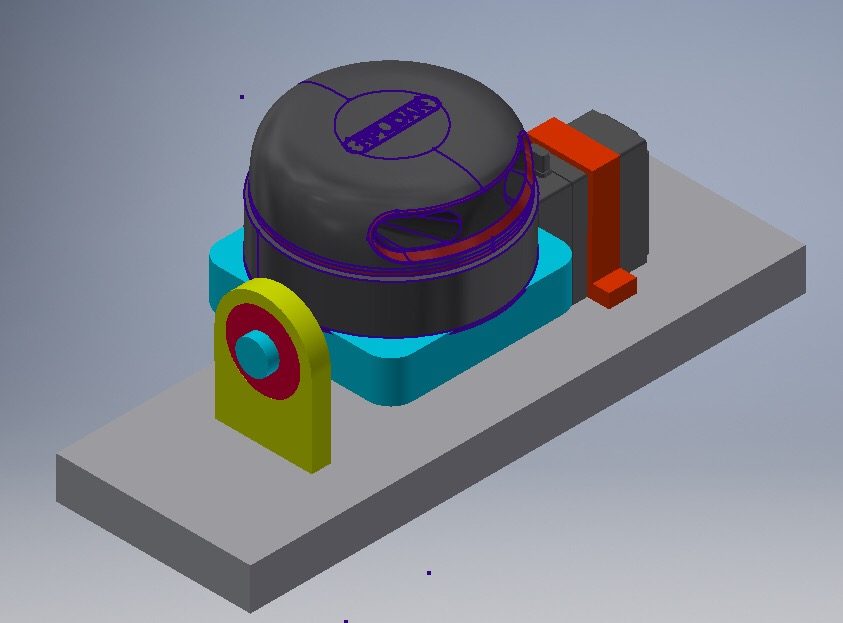
\includegraphics[width=0.16\textwidth]{images/lidar_3D.jpeg}}
  %~\subfloat[Repulsive Force]{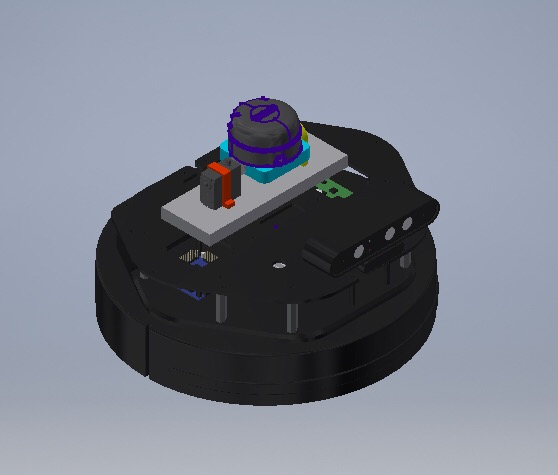
\includegraphics[width=0.16\textwidth]{images/kbki_lidar3D.jpeg}} 
  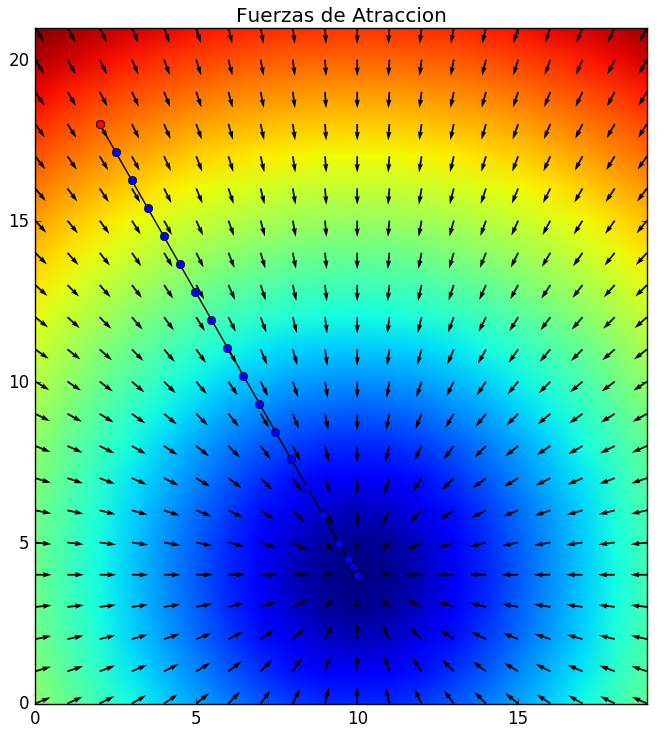
\includegraphics[width=0.40\textwidth]{images/f_attrac.png}
  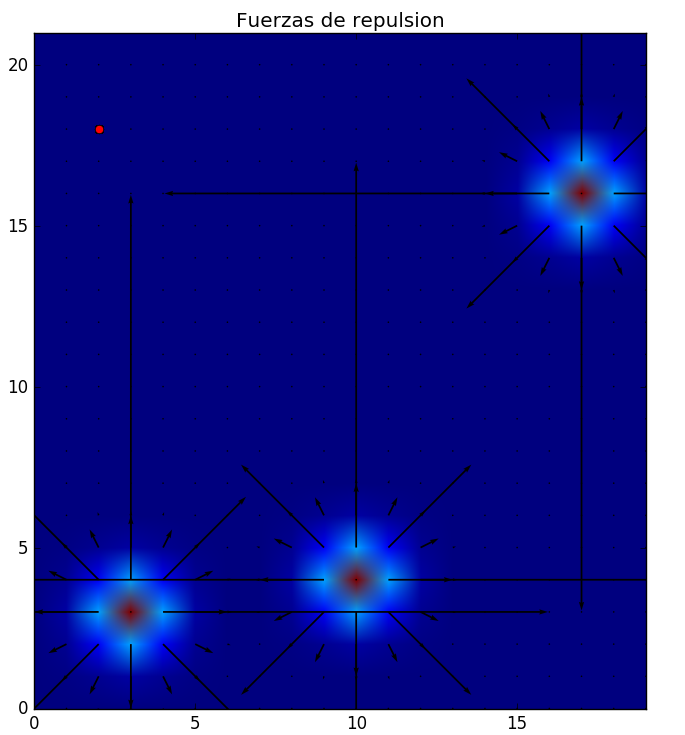
\includegraphics[width=0.41\textwidth]{images/f_reps.png}
  \\ $\qquad\qquad$ a. Sistema mecánico  $\qquad\qquad\qquad$  b. Sistema mecánico encima del Kobuki
  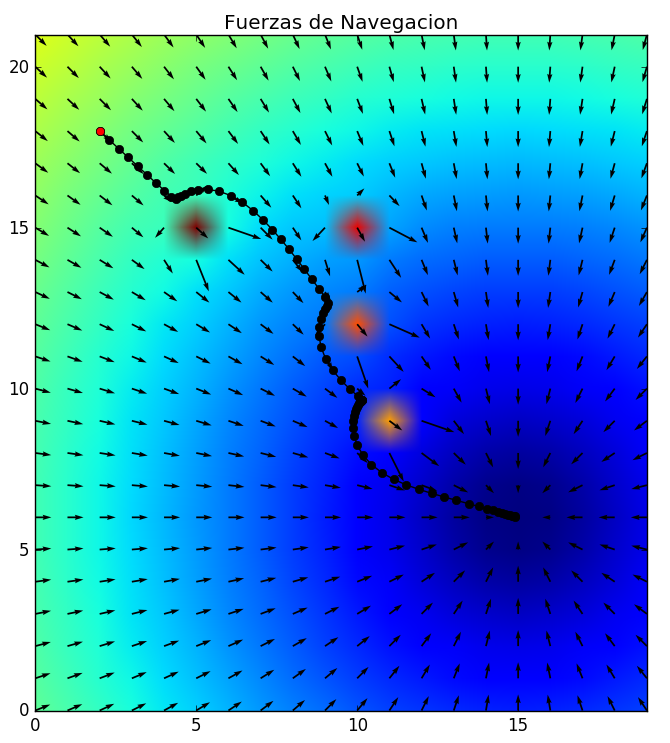
\includegraphics[width=0.40\textwidth]{images/f_nav.png}
  %\subfloat[Navigation Force]{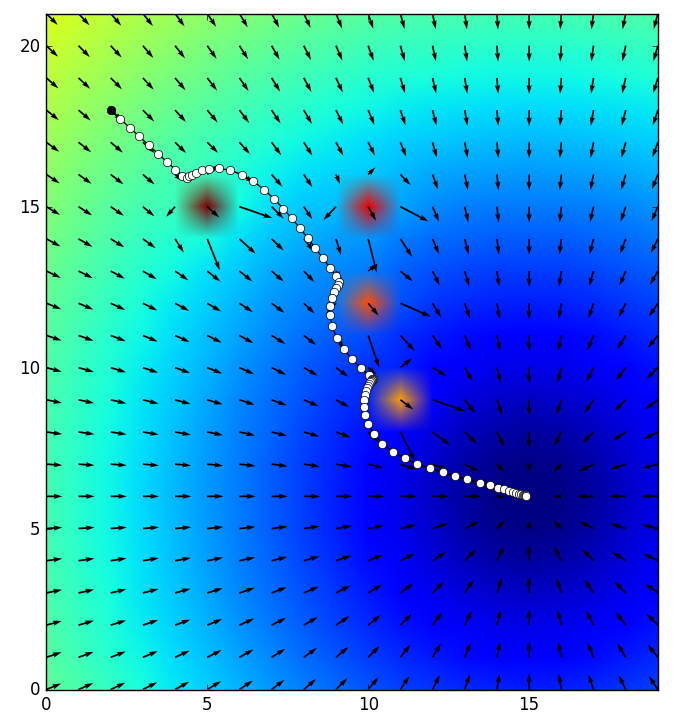
\includegraphics[width=0.16\textwidth]{images/nav_force.png}}
  % \subfloat[Attractive Force]{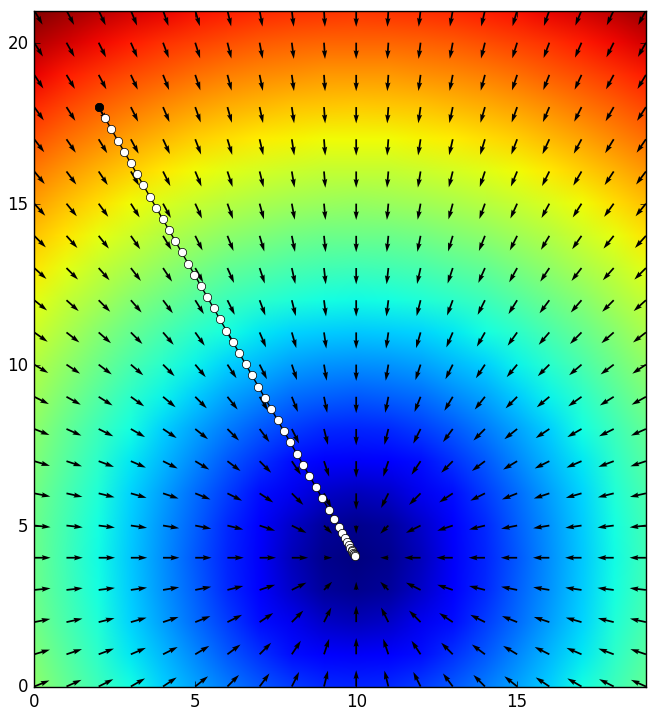
\includegraphics[width = 150mm]{attr_force.png}}
  \captionsetup{font=footnotesize}
  \caption{Sistema mec\'anico para el mapeo en tres dimensiones.}
  %\label{f:lidar3D}
\end{figure}
\subsection{SLAM basado en Filtros de Part\'iculas}

\section{Implementaci\'on del sistema}

\subsection{Sistema Operativo del Robot (ROS)}
ROS es un framework que se usa ampliamente en rob\'otica. Lo que busca 
este sistema operativo de código abierto es hacer una pieza de software 
que pueda funcionar en otros robots con solo pequeños cambios en el 
c\'odigo. Lo que obtenemos con esta idea es la capacidad de crear 
funcionalidades que se pueden compartir y usar en otros robots, por 
lo que no necesitamos volver a reinventar la rueda.

ROS fue desarrollado originalmente en el 2007 por el laboratorio de 
Inteligencia Artificial de Stanford (\textit{SAIL}) en apoyo del proyecto 
Stanford AI Robot \cite{rosHistory}. A partir del 2008, el desarrollo 
contin\'ua principalmente en Willow Garage, un instituto de Investigaci\'on 
de Rob\'otica, con m\'as de veinte instituciones colaborando dentro de un 
modelo de desarrollo federado.

Muchas instituciones de investigaci\'on han comenzado a desarrollarse en 
ROS, agregando hardware y compartiendo su c\'odigo. Los sensores y actuadores 
utilizados en la rob\'otica tambi\'en se han adaptado para su uso en ROS. Gracias 
a esto, las empresas est\'an creando sensores m\'as baratos y m\'as potentes. Arduino 
es un buen ejemplo de esto, ya que al usar una placa electr\'onica barata puede 
agregar una gran cantidad de sensores como codificadores, sensores de luz, 
temperatura, y as\'i sucesivamente \cite{rosIntroduction}.

ROS proporciona las instalaciones del sistema operativo est\'andar, como 
la abstracci\'on de hardware, el control de dispositivos de bajo nivel, la 
implementaci\'on de funcionalidades de uso com\'un, el paso de mensajes entre 
procesos y la gesti\'on de paquetes. %Esta tesis es desarollada con librer\'ias 
%de ROS.

\subsection{Arquitectura del Sistema}


%\section{Hardware usado}
%En esta sección se explicará los componentes que se utilizó para realizar el proyecto. Se comenzará describiendo el quadcopter, posteriormente el sensor láser que fue utilizado, el microcontrolador donde fue implementado el algoritmo SLAM y finalmente del controlador de vuelo Pixhawk.

%\subsection{Fantom}
%Fantom es el quadcopter que fue desarrollado en el laboratorio de robótica de la Universidad de Ingeniería y Tecnología - UTEC, en el año 2015 (Figura \ref{f:fantom}). Este drone fue construído de forma experimental utilizando los motores del DJI Phantom 2; tiene un peso de aproximadamente 1100 gramos (incluyendo batería) y puede cargar 1000 gramos más según las características de sus motores y las pruebas realizadas en el laboratorio. Fantom fue construído para fines aplicativos orientado a métodos de control no lineal.Este drone esta compuesto por:

%\begin{itemize}
%\item[•] Quadcopter Frame fibra de vidrio de 480 mm.
%\item[•] Multi-Rotor Lipo 4S de 4000 mAh.
%\item[•] Multi-Rotor ESC 4S ~ 6S de 20 A.
%\item[•] Motores Brushless 960KV.
%\item[•] Controlador de vuelo Pixhawk.
%\end{itemize}
%\begin{figure}[htb]
%\centering
%\subfloat[Original Image]{\includegraphics[width=40mm]{frame.jpg}}
%~\subfloat[Edges using Canny]{\includegraphics[width=40mm]{bateria.jpg}}\\
%~\subfloat[Dilate Image]{\includegraphics[width=40mm]{dilation_taza.jpg}}
%\subfloat[Morphologically closed image]{\includegraphics[width=40mm]{ESC.jpg}}
%~\subfloat[Skeletonized image]{\includegraphics[width=40mm]{motor.jpg}}
%\subfloat[Morphologically closed image]{\includegraphics[width=40mm]{pixhawk.jpg}}
%\caption{Image processing steps for a 3D real scene} \label{f:cup}
%\end{figure}
%\begin{figure}
%\centering
%\includegraphics[scale=0.1]{fantom.jpg}
%\caption{Quadcopter Fantom.}
%\label{f:fantom}
%\end{figure}

%\subsection{RPLIDAR A2}

%\subsection{Sensor IMU}
%El controlador de vuelo consta de un sensor IMU (acelerómetro, giroscopio y magnetómetro). InvenSense MPU6000 es el sensor IMU y ST Micro L3GD20H + LSM303D o InvenSense ICM2076 actúan como sensores de respaldo \cite{pixhawkIMU}. El primer conjunto de sensores se coloca en la placa primaria de la FCU mientras que el tercer conjunto se coloca en la placa aislada de las vibraciones. Las lecturas de estos diferentes conjuntos de sensores se colocan en buses separados. Son responsables de proporcionar la medición inercial necesaria para maniobrar el quadcopter. Las lecturas del giroscopio que indican la rotación de las aeronaves sobre sus propios ejes son necesarias para un vuelo estable, utilizado internamente por el controlador PID. Las lecturas del acelerómetro proporcionan las fuerzas de aceleración y aceleración en los 3 ejes, ayudan en el control de la posición de la aeronave. Esta información se puede utilizar para la estimación de la posición, pero se sabe que es propensa a errores. El magnetómetro o la brújula es responsable de proporcionar información sobre el campo magnético de la tierra e inferir el norte magnético.

%\subsection{Sensor Barométrico}
%El controlador de vuelo consta de 2 sensores barométricos MS5611 redundantes. Mide la presión del aire y, en teoría, se puede utilizar para predecir la altitud, pero necesita una recalibración frecuente.
 
%\subsection{Controlador de Vuelo}
%Pixhawk \cite{PixhawkHome}, fabricado por Proficnc es la unidad de controlador de vuelo a bordo del quadcopter que vamos a utilizar en este proyecto (Figura \ref{f:pixhawk}). La función de este dispositivo es leer los datos de entrada de los sensores (láser e IMU), realizar cálculos y, como resultado, manipular la velocidad de los motores para ejecutar las manibras necesarias. Es un piloto automático de código abierto donde los desarrolladores se encargan de compartir en los repositorios de Ardupilot \cite{Ardupilot}. Para mejorar las lecturas del sensor IMU, el Pixhawk viene con 3 sistemas IMU redundantes, que están aislados entre sí, y también están amortiguados para evitar que las vibraciones del vuelo corrompan los datos.

%El Pixhawk viene con un IMU desacoplado y FMU (unidad de gestión de vuelo) para reducir la interferencia a los sensores. Tiene un núcleo ARM Cortex M4 de 32 bits con FPU que opera a una frecuencia de 168 Mhz, 256 KB RAM, memoria flash de 2 MB y un coprocesador a prueba de fallos de 32 bits (REFERENCIAR DATASHEET). Los sensores a bordo se discute a detalle en las subsecciones 3.2.3 y 3.2.4.
%El Pixhawk viene con un solo suministro independiente de 5V para el controlador de vuelo y sus periféricos. También proporciona protección contra sobre voltaje, protección contra sobrecorriente y protección térmica. La FMU y la IO (entradas y salidas) funcionan a 3.3V y 6.6V. Se puede alimentar a través de USB o a través de los 2 conectores. Para las operaciones IO, viene con un puerto I2C, 2 puertos CAN, 5 puertos UART, un puerto SPI y un puerto RSSI (PWM o Voltaje).

%\begin{figure}
%\centering
%\includegraphics[scale=0.4]{pixhawk.jpg}
%\caption{Controlador de Vuelo Pixhawk}
%\label{f:pixhawk}
%\end{figure}

%\section{Arquitectura de Solución}
%\subsection{Arquitectura del Sistema}
%\subsection{HectorSlam}
%\subsection{Mavros}

